%%%%%%%%%%%%%%%%%%%%%%%%%%%%%%%%%%%%%%%%%
% Short Sectioned Assignment LaTeX Template Version 1.0 (5/5/12)
% This template has been downloaded from: http://www.LaTeXTemplates.com
% Original author:  Frits Wenneker (http://www.howtotex.com)
% License: CC BY-NC-SA 3.0 (http://creativecommons.org/licenses/by-nc-sa/3.0/)
%%%%%%%%%%%%%%%%%%%%%%%%%%%%%%%%%%%%%%%%%

%----------------------------------------------------------------------------------------
%	PACKAGES AND OTHER DOCUMENT CONFIGURATIONS
%----------------------------------------------------------------------------------------

\documentclass[paper=a4, fontsize=11pt]{scrartcl} % A4 paper and 11pt font size

% ---- Entrada y salida de texto -----

\usepackage[T1]{fontenc} % Use 8-bit encoding that has 256 glyphs
\usepackage[utf8]{inputenc}

% ---- Idioma --------

\usepackage[spanish, es-tabla]{babel} % Selecciona el español para palabras introducidas automáticamente, p.ej. "septiembre" en la fecha y especifica que se use la palabra Tabla en vez de Cuadro

% ---- Otros paquetes ----

\usepackage{amsmath,amsfonts,amsthm} % Math packages
\usepackage{graphics,graphicx, floatrow} %para incluir imágenes y notas en las imágenes
\usepackage{graphics,graphicx, float} %para incluir imágenes y colocarlas
\usepackage{hyperref} % url in references

% Para hacer tablas comlejas
\usepackage{multirow}
\usepackage{threeparttable}

\usepackage{fancyhdr} % Custom headers and footers
\pagestyle{fancyplain} % Makes all pages in the document conform to the custom headers and footers
\fancyhead{} % No page header - if you want one, create it in the same way as the footers below
\fancyfoot[L]{} % Empty left footer
\fancyfoot[C]{} % Empty center footer
\fancyfoot[R]{\thepage} % Page numbering for right footer
\renewcommand{\headrulewidth}{0pt} % Remove header underlines
\renewcommand{\footrulewidth}{0pt} % Remove footer underlines
\setlength{\headheight}{13.6pt} % Customize the height of the header

\numberwithin{equation}{section} % Number equations within sections (i.e. 1.1, 1.2, 2.1, 2.2 instead of 1, 2, 3, 4)
\numberwithin{figure}{section} % Number figures within sections (i.e. 1.1, 1.2, 2.1, 2.2 instead of 1, 2, 3, 4)
\numberwithin{table}{section} % Number tables within sections (i.e. 1.1, 1.2, 2.1, 2.2 instead of 1, 2, 3, 4)

\setlength\parindent{0pt} % Removes all indentation from paragraphs - comment this line for an assignment with lots of text

\newcommand{\horrule}[1]{\rule{\linewidth}{#1}} % Create horizontal rule command with 1 argument of height

\usepackage{textcomp}

%----------------------------------------------------------------------------------------
%	DATOS
%----------------------------------------------------------------------------------------

\newcommand{\myName}{Francisco Javier Bolívar Lupiáñez}
\newcommand{\myDegree}{Máster en Ingeniería Informática}
\newcommand{\myFaculty}{E. T. S. de Ingenierías Informática y de Telecomunicación}
\newcommand{\myDepartment}{Ciencias de la Computación e Inteligencia Artificial}
\newcommand{\myUniversity}{\protect{Universidad de Granada}}
\newcommand{\myLocation}{Granada}
\newcommand{\myTime}{\today}
\newcommand{\myTitle}{Práctica 1}
\newcommand{\mySubtitle}{Redes neuronales. Reconocimiento óptico de caracteres MNIST}
\newcommand{\mySubject}{Inteligencia Computacional}
\newcommand{\myYear}{2016-2017}

%----------------------------------------------------------------------------------------
%	PORTADA
%----------------------------------------------------------------------------------------


\title{	
	\normalfont \normalsize 
	\textsc{\textbf{\mySubject \space (\myYear)} \\ \myDepartment} \\[20pt] % Your university, school and/or department name(s)
	\textsc{\myDegree \\[10pt] \myFaculty \\ \myUniversity} \\[25pt]
	\horrule{0.5pt} \\[0.4cm] % Thin top horizontal rule
	\huge \myTitle: \mySubtitle \\ % The assignment title
	\horrule{2pt} \\[0.5cm] % Thick bottom horizontal rule
	\normalfont \normalsize
}

\author{\myName} % Nombre y apellidos

\date{\myTime} % Incluye la fecha actual
%----------------------------------------------------------------------------------------
%	INDICE
%----------------------------------------------------------------------------------------

\begin{document}
	
\setcounter{page}{0}

\maketitle % Muestra el Título
\thispagestyle{empty}

\newpage %inserta un salto de página

\tableofcontents % para generar el índice de contenidos

%\listoffigures

\newpage

%----------------------------------------------------------------------------------------
%	DOCUMENTO
%----------------------------------------------------------------------------------------

\section{Introducción}

Las redes neuronales son muy utilizadas para el reconocimiento de patrones. Y se podría decir que el ``Hola mundo'' de éstas es la base de datos MNIST \footnote{\url{http://yann.lecun.com/exdb/mnist/}} para el Reconocimiento Óptico de Caracteres (OCR).
\\ \\
Esta base de datos contiene 60.000 imágenes de números (Figura \ref{fig:sample-mnist-data}) para entrenar la red neuronal y 10.000 para probarla. Cada una de estas imágenes de un tamaño de 28x28 píxeles.
\begin{figure}[H]
	\centering
	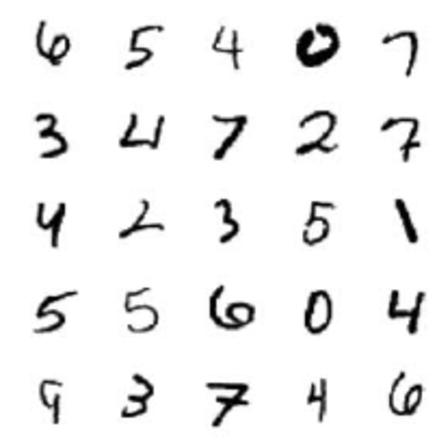
\includegraphics[width=6cm]{img/sample-mnist-data}
	\caption{Muestra de algunas de las imágenes de números de la base de datos MNIST}
	\label{fig:sample-mnist-data}
\end{figure}
El objetivo de esta práctica es el estudio del uso de distintas redes neuronales para resolver este problema obteniendo el mínimo porcentaje de error posible.
\\ \\
Para ello, se ha realizado durante varias semanas de clase una introducción desde cero de los distintos métodos que podrían utilizarse. Desde un perceptrón simple hasta redes neuronales convolucionales.

\section{Implementación}

La primera decisión que tuve que tomar fue la de qué lenguaje de programación y librerías utilizar. 
\\ \\
Me hacía ilusión \textbf{realizar una red neuronal sin la ayuda de ninguna librería}, por lo que descarté desde un principio la posibilidad de utilizar alguna librería que me pudiese facilitar el trabajo. 
\\ \\
Dado que se proporcionaron algoritmos para la lectura de los datos de MNIST tanto en Java y MatLab, y no conocía ni había usado antes MatLab, \textbf{decidí usar Java}, un lenguaje de programación que domino con soltura después de varios años de experiencia utilizando para distintas prácticas del grado en ingeniería informática.

\subsection{Una primera solución: plantillas}

La primera solución que probé para resolver el problema, fue la idea que se presentó el primer día de clase, que trataba de \textbf{crear plantillas según las imágenes de entrenamiento}.
\\ \\
Para entrenar, se recorre cada imagen de entrenamiento y, para cada píxel de la imagen, se ve si tiene tinta o no. Si la tiene, se le suma valor a ese píxel en la plantilla con el mismo índice que la etiqueta de la imagen que se está utilizando para entrenar. Si por el contrario no tiene tinta, lo que se hace es restar.
\\ \\
Una vez entrenada, para ver cuál es el número de una imagen de test, por cada píxel con tinta, se ve si se tiene un valor positivo en cada una de las plantillas, y para el que tenga, se le añade un voto. Una vez recorridos todos los píxeles de la imagen, se hace un recuento de votos, y la plantilla que haya obtenido más votos es la que indica el número que se ve en la imagen.
\\ \\
Esta solución. Al iniciar siempre a cero los valores de las plantillas generaba siempre el mismo \textbf{resultado que era el de un 55,8\%}.
\\ \\
Esta tasa de error \textbf{se redujo hasta un 34,09\% al reforzar los píxeles con tinta} sumando 5 en vez de 1 a la plantilla.

\subsection{\textit{Backpropagation}}

La falta de tiempo por la proximidad de la fecha de entrega tras haber dejado aparcada la práctica varias semanas hizo que pasase directamente de esta primera y muy básica solución a la realización de algo que pudiese bajar del 10\% de error. Por lo que pasé de realizar el perceptrón simple con el que obtendría unos resultados similares a los ya obtenidos y me puse manos a la obra con una red neuronal multicapa con \textit{backpropagation}.

\subsubsection{\textit{Backpropagation} simple con una sola época}

Realicé una primera implementación con la siguiente topología:
\begin{itemize}
	\item \textbf{Número de capas}: Tres capas. Capa de entrada, oculta y de salida
	\item \textbf{Tamaño de capa de entrada}: 28x28. Tantas neuronas como píxeles en la imagen
	\item \textbf{Tamaño de capa de salida}: 10. Tantas neuronas como posibles soluciones. Si tiene valor 1, o lo ronda, significará que el número de la imagen corresponde al índice de esa neurona
	\item \textbf{Pesos}: Un peso por cada conexión entre neurona inicializados entre -1,67 y 1,67
	\item \textbf{Función de activación}: Sigmoidal
	\item \textbf{Ratio de aprendizaje}: 0,7
	\item \textbf{Tipo de aprendizaje}: Estocástico. Reajuste de pesos tras cada imagen
\end{itemize}
Los resultados obtenidos tras una sola época eran malos, rondaban el 90\%. Y no solo era por inicializar los pesos de las neuronas a unos valores tan grandes, ni por ese ratio excesivamente grande. El problema era que había calculado mal las funciones utilizadas para reajustar los pesos.
\\ \\
Para solucionar esto estuve leyendo varios artículos \cite{backpropagation-de} \cite{backpropagation-au} que me ayudaron a encontrar los fallos que tenía. Antes de empezar a depurar los fallos, cambié el número de neuronas en la capa oculta para que el tiempo de entrenamiento fuese más corto y usé 100 neuronas en ésta capa.
\\ \\
Una vez resueltos estos fallos, añadido el sesgo y su peso (\textit{bias}) a cada neurona y cambiado los valores tanto de inicialización de los pesos (-0,1 y 0,1) y el ratio de aprendizaje (0,17), en una sola época se obtuvo un \textbf{resultado que rondó el 10\%}.

\subsubsection{\textit{Backpropagation} usando momentos y varias épocas}

Para mejorar los resultados podía aplicar \textit{softmax}, pero el tiempo con el que contaba era escaso, por lo que el siguiente paso que podía dar sin agotar mucho tiempo era el del uso de momentos.
\\ \\
No obstante, el uso que hice de este método no es el que se hace de él normalmente. Pues en lugar de variar el valor del momento de 0,5 al principio hasta 0,9 lo iniciaba directamente a 0,9. No se aprovecha de esta forma todas las ventajas que se podrían llegar a tener durante la oscilación en el gradiente descendente, pero sí mejoraba los resultados \textbf{de en torno a un 4\% tras diez épocas con la topología anterior} (con 256 neuronas en la capa oculta) \textbf{a un 2\%} solo añadiendo la constante del momento, multiplicada por la variación del peso anterior, a la variación del peso actual \cite{backpropagation-au}.

\subsection{Topología de la red neuronal final}

La red neuronal final se podría definir como una red neuronal multicapa, que usa una función de activación sigmoidal, \textit{backpropagation} con momentos y aprendizaje estocástico.

\begin{figure}[H]
	\centering
	\includegraphics[width=14.5cm]{img/neural-network}
	\caption{Esquema gráfico de la red neuronal propuesta}
	\label{fig:neural-network}
\end{figure}

\subsubsection{\textit{Feed forward propagation}}

Las salidas de la primera capa serán las entradas de la red neuronal, correspondientes a los valores de cada uno de los píxeles de la imagen.

Para calcular la salida durante la \textit{feed forward propagation} en la capa \textit{k} y la neurona \textit{i} se usa la siguiente función:

\[ x^{(k)}_{i} = \sum_{j=0}^{k_{size}-1}(w^{(k)}_{i,j} O^{(k-1)}_{j}) + \theta^{(k)}_{i} \]

donde:
\begin{itemize}
	\item $ w^{(k)}_{i,j} $ es el peso de la conexión entre la neurona \textit{i} de la capa \textit{k} y la neurona \textit{j} de la capa \textit{k-1}
	\item $ O^{(k-1)}_{j} $ es la salida de la neurona \textit{j} en la capa \textit{k-1}
	\item $ \theta^{(k)}_{i} $ es el peso del \textit{bias} en la neurona \textit{i} de la capa \textit{k}
\end{itemize}

Y a este resultado se le aplica la función sigmoidal:

\[O^{(k)}_{i} = \dfrac{1}{1 + e^{x^{(k)}_{i}}} \]

\subsubsection{\textit{Backpropagation} en la capa de salida}

Para calcular la variación de los pesos, en primer lugar, hay que calcular la señal de error:

\[ \delta^{(k)}_{i} = (t^{(k)}_{i} - O^{(k)}_{i}) O^{(k)}_{i} (1 - O^{(k)}_{i}) \]

donde:
\begin{itemize}
	\item $ t^{(k)}_{i} $ es el valor objetivo de la neurona \textit{i} de la capa \textit{k}
	\item $ O^{(k)}_{i} $ es la salida de la neurona \textit{i} en la capa \textit{k}
\end{itemize}

Con la señal de error calculada se puede calcular la variación del peso:

\[ \Delta w^{(k)}_{i,j} = \delta^{(k)}_{i} O^{(k-1)}_{j} \eta + \Delta w^{(k)}_{i,j} \mu \]

donde:
\begin{itemize}
	\item $ \delta^{(k)}_{i} $ es la señal de error calculada anteriormente
	\item $ O^{(k-1)}_{j} $ es la salida de la neurona \textit{j} en la capa \textit{k-1}
	\item $ \Delta w^{(k)}_{i,j} $ es la variación anterior de ese peso
	\item $ \eta $ es el ratio de aprendizaje
	\item $ \mu $ es el valor del momento
\end{itemize}

Y finalmente, para calcular el nuevo valor del peso, solo hay que sumar la variación calculada al peso actual.

\[ w^{(k)}_{i,j} = w^{(k)}_{i,j} +\Delta w^{(k)}_{i,j} \]

\subsubsection{\textit{Backpropagation} en la capa oculta}

Para calcular la variación del peso en la capa oculta, lo único que cambiaría con respecto a lo descrito anteriormente para la capa de salida es la señal de error ya que no se conocen los valores objetivos de las neuronas en la capa oculta:

\[ \delta^{(k)}_{i} = \sum_{j=0}^{(k+1)_{size}-1}(\delta^{(k+1)}_{j} w^{(k+1)}_{i,j}) O^{(k)}_{i} (1 - O^{(k)}_{i}) \]

\subsection{Ajuste de parámetros}

Una vez definida la red neuronal, queda ajustar los parámetros para obtener el mejor resultado posible.
\\ \\
Los parámetros a ajustar son:
\begin{itemize}
	\item Neuronas en la capa oculta
	\item Tasa de aprendizaje
	\item Número de épocas
\end{itemize}

Para ello se han realizado experimentos para ver cómo funcionan todos estos parámetros y cómo se relacionan los unos con los otros.

\subsubsection{Número de neuronas en la capa oculta y épocas}

Se han realizado pruebas con capas ocultas de 100, 200, 300 y 400 neuronas, de 5, 10, 15, 20, 25, 30, 35, 40, 45 y 50 épocas con un valor fijo en la tasa de aprendizaje de 0,017.

\begin{table}[H]
\centering
\caption{Porcentaje de error según número de neuronas en la capa oculta y número de épocas}
\label{tab:hidden-size-and-epochs}
\begin{tabular}{| c | c | c | c | c |}
	\hline
	   & 100  & 200  & 300  & 400  \\ 
	\hline
	5  & 3,00 & 2,70 & 2,47 & 2,39 \\
	10 & 2,46 & 2,27 & 2,10 & 2,01 \\
	15 & 2,21 & 2,05 & 1,93 & 1,85 \\
	20 & 2,22 & 1,91 & 1,80 & 1,77 \\
	25 & 2,23 & 1,92 & 1,74 & 1,71 \\
	30 & 2,26 & 1,92 & 1,74 & 1,70 \\
	35 & 2,25 & 1,91 & 1,75 & 1,70 \\
	40 & 2,28 & 1,91 & 1,76 & 1,72 \\
	45 & 2,27 & 1,92 & 1,75 & 1,70 \\
	50 & 2,26 & 1,93 & 1,76 & 1,72 \\ 
	\hline
\end{tabular}
\end{table}

\begin{figure}[H]
	\centering
	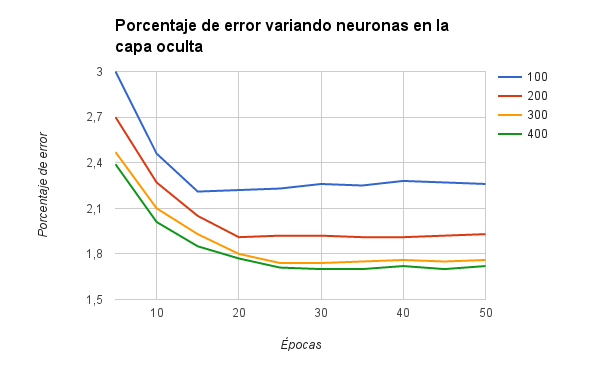
\includegraphics[width=14cm]{img/hidden-size-and-epochs}
	\caption{Gráfico con el porcentaje de error según número de neuronas en la capa oculta y número de épocas}
	\label{fig:hidden-size-and-epochs}
\end{figure}

Con este pequeño experimento se han podido sacar varias conclusiones. 
\begin{itemize}
	\item A mayor número de neuronas en la capa oculta mejor resultado en cuanto a porcentaje de error
	\item A mayor número de neuronas en la capa oculta más épocas se necesitan para que aprendan
\end{itemize}

\subsubsection{Número de neuronas en la capa oculta y tiempo de ejecución}

Aunque en un principio el tiempo de ejecución no es algo crítico, pues se puede dejar a la red neuronal aprendiendo durante horas o días, para esta práctica voy a utilizar un tamaño con el que los tiempos de ejecución sean razonables y no tenga que tener el ordenador conectado un día entero mientras la neurona está aprendiendo.
\\ \\
Por lo que se ha medido el tiempo de ejecución de una época para capas ocultas con 100, 200, 300, 400, 500, 600, 700 y 800 neuronas.
\begin{table}[H]
	\centering
	\caption{Tiempo de entrenamiento con una una sola época variando neuronas en la capa oculta}
	\label{tab:one-epoch-run-time}
	\begin{tabular}{| c | c |}
		\hline
		capa oculta & tiempo (seg.) \\ 
		\hline
		100 & 21 \\
		200 & 40 \\
		300 & 62 \\
		400 & 84 \\
		500 & 115 \\
		600 & 145 \\
		700 & 171 \\
		800 & 191 \\
		\hline
	\end{tabular}
\end{table}

\begin{figure}[H]
\centering
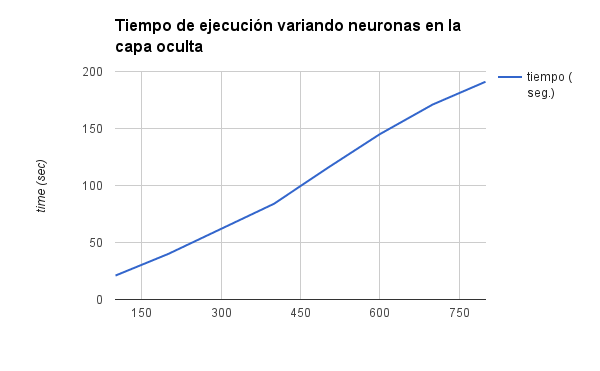
\includegraphics[width=14cm]{img/one-epoch-run-time}
\caption{Gráfico con el tiempo de entrenamiento con una sola época variando neuronas en la capa oculta}
\label{fig:one-epoch-run-time}
\end{figure}

El comportamiento que sigue es más o menos lineal y, visto que una época con 800 neuronas en la capa oculta ronda los tres minutos y\textbf{ la capa de entrada es de 784, le voy a dar el mismo número de neuronas a la capa oculta}, por lo que un entrenamiento de 50 épocas rondaría las dos horas y media.

\subsubsection{Tasa de aprendizaje}

Los experimentos utilizados hasta ahora han sido utilizando una tasa de aprendizaje de 0,017. Se sabe que a menor sea la tasa de aprendizaje mayor será el número de épocas necesarias para aprender. Y ya que no se quiere exceder mucho el tiempo de ejecución, no se usarán tasas de aprendizaje demasiado pequeñas. Ni tampoco tan grandes como para que sobreaprenda en pocas épocas.
\\ \\
Se calculará la tasa de error tras 30 épocas en una red neuronal con 768 neuronas ocultas, para tasas de aprendizaje de 0,005, 0,01, 0,05 y 0,1 para ver si la tasa de aprendizaje fijada hasta ahora está en un rango con el que se producen resultados apropiados.
\begin{table}[H]
	\centering
	\caption{Porcentaje de error variando tasa de aprendizaje}
	\label{tab:learning-rate}
	\begin{tabular}{| c | c | c | c | c |}
		\hline
		  & 0,005 & 0,01 & 0,05 & 0,1  \\ 
		\hline
		5  & 3,81 & 2,78 & 2,27 & 3,40 \\
		10 & 2,73 & 2,15 & 2,09 & 3,14 \\
		15 & 2,29 & 1,91 & 1,81 & 2,96 \\
		20 & 2,05 & 1,81 & 1,74 & 2,67 \\
		25 & 2,00 & 1,76 & 1,68 & 2,71 \\
		30 & 1,97 & 1,68 & 1,69 & 2,68 \\
		35 & 1,95 & 1,64 & 1,68 & 2,66 \\
		40 & 1,85 & 1,64 & 1,67 & 2,71 \\
		45 & 1,80 & 1,65 & 1,68 & 2,73 \\
		50 & 1,79 & 1,66 & 1,69 & 2,72 \\ 
		\hline
	\end{tabular}
\end{table}

\begin{figure}[H]
\centering
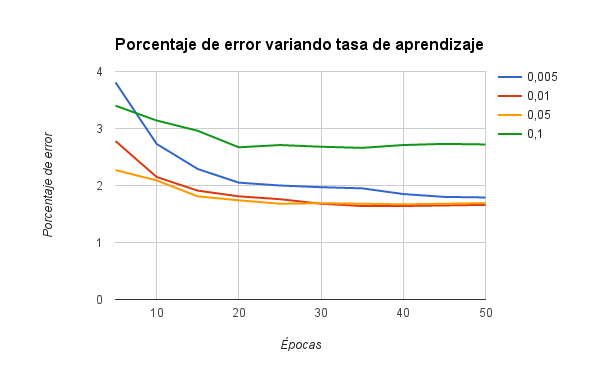
\includegraphics[width=14cm]{img/learning-rate}
\caption{Gráfico con el porcentaje de error variando tasa de aprendizaje}
\label{fig:learning-rate}
\end{figure}

Se puede ver cómo con la tasa de aprendizaje más pequeña (0,001), en 50 épocas no se llega a obtener todavía el resultado óptimo, pues todavía estaba bajando el porcentaje de error cuando se paró la ejecución. Y como se estudió antes, más de 50 épocas puede implicar más de dos horas y media, por lo que se optará por una tasa de aprendizaje algo más grande.
\\ \\
Con la tasa de aprendizaje más alta (0,1) sobreaprende demasiado pronto obteniendo los peores resultados.
\\ \\
Con las tasas que mejor se comporta es con las intermedias (0,01 y 0,05). Con las más alta de las dos necesita menos épocas para estabilizarse, pero obtiene un peor resultado que con la más baja de éstas, que aunque necesita diez épocas más para obtener su mejor resultado, éste mejora en tres centésimas al mejor obtenido con la otra.
\\ \\
La diferencia no es muy alta, por lo que \textbf{una tasa de aprendizaje entre 0,01 y 0,05 es la ideal} en esta red neuronal con los parámetros establecidos anteriormente para obtener el mejor resultado en menos de 50 épocas.

\subsubsection{Número de épocas}

Para ver el número de épocas necesario lo que se hará es ir comprobando el porcentaje de error que se obtendría cada vez que se actualizan los pesos, y si es menor que el menor obtenido hasta el momento, exportar esos pesos. De esta forma, aunque el tiempo de ejecución sea muy elevado, se podrá dejar trabajando solo sabiendo que se extraerá el mejor de los pesos encontrados durante un número de épocas que se ha fijado en 50.
\\ \\
Si se monitoriza, se ve que se ha estancado y deja de mejorar; se corta la ejecución para que no realice las épocas restantes.
\\ \\
De esta forma. Con 784 neuronas en la capa oculta y un ratio de aprendizaje de 0,017 \textbf{se ha obtenido el mejor resultado sobre las imágenes de test en 33 épocas} (1,63\% de error y 0,32\% sobre el conjunto de imágenes de entrenamiento).

\section{Resultados}

En esta sección voy a presentar una tabla con los resultados que fui obteniendo con las distintas redes neuronales que he ido desarrollando hasta llegar a obtener mi mejor resultado (Tabla \ref{tab:results}).

\begin{table}[H]
	\centering
	\caption{Resultados obtenidos durante el transcurso de la práctica}
	\label{tab:results}
	\begin{tabular}{| l | c | c | c | c |}
		\hline
		Versión & Épocas & Neuronas en capa oculta & $\eta$ & \% Error \\ 
		\hline
		Plantillas & 1 & - & - & 55,8 \\
		Plantillas con refuerzo & 1 & - & - & 34,09 \\
		\textit{Backpropagation} & 1 & 784 & 0,1 & 9,8 \\
		\textit{Backpropagation} & 25 & 100 & 0,017 & 3,4 \\
		\textit{Backpropagation} & 25 & 400 & 0,017 & 2,15 \\
		\textit{Backpropagation} con momentos & 25 & 400 & 0,017 & 1,71 \\
		\textit{Backpropagation} con momentos & 33 & 784 & 0,017 & 1,63 \\
		\hline
	\end{tabular}
\end{table}

\section{Conclusiones}

Con esta práctica he podido iniciarme en el mundo del reconocimiento de patrones realizando una especie de ``Hola mundo'' usando la base de datos de MNIST para reconocer dígitos con una red neuronal implementada en Java desde cero.
\\ \\
El transcurso de esta práctica ha sido una auténtica montaña rusa. Desde los momentos más bajos cuando la red neuronal no funcionaba y no bajaba del 20\% de error cuando debería rozar el 10\%, hasta los momentos de euforia cuando conseguía reducir poco a poco la tasa de error.
\\ \\
Estoy tremendamente orgulloso de haber conseguido estos resultados. Sobre todo, por haberlo hecho sin hacer uso de ninguna librería. No obstante, me habría gustado tener tiempo para mirar varias librerías con las que, usando otras técnicas como \textit{softmax} o redes neuronales convolucionales. Así mismo, me habría gustado paralelizar usando CUDA los algoritmos de \textit{feed forward propagation} y \textit{back propagation}.
\\ \\
Sin embargo, lo más positivo no es el haber realizado esta práctica con éxito sino el descubrimiento de una técnica que puede ser muy útil para resolver problemas que hace unos meses no sabría como resolver de forma eficaz y eficiente.


%----------------------------------------------------------------------------------------
%	REFERENCIAS
%----------------------------------------------------------------------------------------

\newpage

\bibliography{referencias} %archivo referencias.bib que contiene las entradas 
\bibliographystyle{plain} % hay varias formas de citar

\end{document}